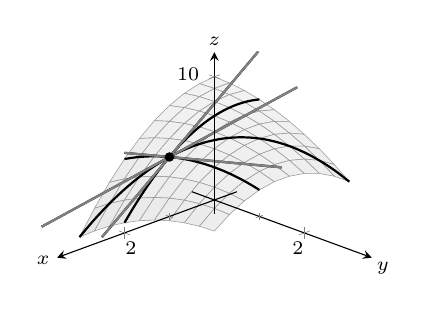
\begin{tikzpicture}[>=stealth]
\begin{axis}%
[width=175pt,tick label style={font=\scriptsize},axis on top,
			axis lines=center,
			view={135}{30},
			name=myplot,
			%xtick=\empty,
			%ytick={5},
			ztick={10},
			minor xtick=1,
			minor ytick=1,
			ymin=-.5,ymax=3.5,
			xmin=-.5,xmax=3.5,
			zmin=-1.1, zmax=12,
			every axis x label/.style={at={(axis cs:\pgfkeysvalueof{/pgfplots/xmax},0,0)},xshift=-5pt,yshift=-1pt},
				xlabel={\scriptsize $x$},
			every axis y label/.style={at={(axis cs:0,\pgfkeysvalueof{/pgfplots/ymax},0)},xshift=4pt,yshift=-4pt},
				ylabel={\scriptsize $y$},
				every axis z label/.style={at={(axis cs:0,0,\pgfkeysvalueof{/pgfplots/zmax})},xshift=0pt,yshift=4pt},
				zlabel={\scriptsize $z$}
			]

%\addplot3[domain=0:180,smooth,y domain=0:360,surf,%fill=white,
%colormap={mp2}{\colormapplaneone},faceted color=black!40,samples=30,samples y=25,very thin,z buffer=sort] ({cos(x)*1.5*cos(y)},{sin(x)*cos(y)},{sin(y)});

\addplot3[domain=0:3,y domain=0:3,surf,colormap={mp2}{rgb=(.9,.9,.9); rgb=(.95,.95,.95)},shader=faceted,faceted color=black!40,samples y=10,very thin,z buffer=sort,
samples=10,] (x,y,{-x^2-.5*(y^2)+x*y+10});

\addplot3 [thick,{\colorone}, smooth,domain=0:3,samples=20,samples y=0] ({x},{1},{-x^2+x+9.5});

\addplot3 [thick,{\colorone}, smooth,domain=0:3,samples=20,samples y=0] ({2},{x},{-.5*x^2+2*x+6});

\addplot3 [thick,{\colorone}, smooth,domain=0:3,samples=20,samples y=0] ({x},{3-x},{-x^2-.5*((3-x)^2)+x*(3-x)+10});

\ifthenelse{\boolean{colorprint}}
{% in color
\addplot3 [thick,{\colortwo}, smooth,domain=-2:2,samples=2,samples y=0] ({-.71*x+2},{.71*x+1},{2.83*x+7.5});
\addplot3 [thick,{\colortwo}, smooth,domain=0:3.5,samples=2,samples y=0] ({2},{x},{1*(x-1)+7.5});
\addplot3 [thick,{\colortwo}, smooth,domain=0:3.5,samples=2,samples y=0] ({x},{1},{-3*(x-2)+7.5});
}
{%not in color
\addplot3 [thick,black!50!white, smooth,domain=-2:2,samples=2,samples y=0] ({-.71*x+2},{.71*x+1},{2.83*x+7.5});
\addplot3 [thick,black!50!white, smooth,domain=0:3.5,samples=2,samples y=0] ({2},{x},{1*(x-1)+7.5});
\addplot3 [thick,black!50!white, smooth,domain=0:3.5,samples=2,samples y=0] ({x},{1},{-3*(x-2)+7.5});

}
\filldraw [black] (axis cs:2,1,7.5) circle (1.5pt);



%\addplot3 [thick,{\colorone}, smooth,domain=-3:3,samples=20,samples y=0] ({x},{2},{x^2+8});
%
%\addplot3 [thick,{\colorone}, smooth,domain=-30:170,samples=60,samples y=0] ({2.93*(cos(x))},{1.96*(sin(x))},.2);
%
%\addplot3 [thick,{\colorone}, smooth,domain=-30:170,samples=60,samples y=0] ({2.75*(cos(x))},{1.83*(sin(x))},.4);
%
%\addplot3 [thick,{\colorone}, smooth,domain=-35:170,samples=60,samples y=0] ({2.4*(cos(x))},{1.6*(sin(x))},.6);
%
%\addplot3 [thick,{\colorone}, smooth,domain=-40:170,samples=60,samples y=0] ({1.8*(cos(x))},{1.2*(sin(x))},.8);
%
%\filldraw [{\colorone}] (axis cs: 0,0,1) circle (1pt);

\end{axis}


\end{tikzpicture}












